% =====================
\section{プロジェクトの概要}

\subsection{プロジェクトの題目}
指揮者人形による自律同期Arduinoオーケストラ

\subsection{プロジェクトの目的}

音楽の自動演奏システムは数多く存在するが，その大半は事前に定義された楽譜とテンポを機械的に再生するに留まり，演奏中の人間的な表現が介在する余地は乏しい．とりわけ，指揮者がリアルタイムに与えるアゴーギク，\textit{accelerando}（加速），\textit{ritardando}（減速），フェルマータ（音の引き伸ばし）といったテンポと時間の揺らぎは，音楽の重要な要素の一つである．Borchersらが Personal Orchestra として実装した研究\cite{borchers2004personal}以降，指揮動作を入力として演奏速度を変更するシステムは複数提案されてきたが，その多くは中央のサーバが指揮を解釈して各音源に同期信号を配信する集中型アーキテクチャを採用しており，人間のオーケストラに見られる「各奏者が指揮者を観測して同期する」という分散的構造とは異なる．

本プロジェクトの目的は，指揮者ロボットの物理的動作を各楽器ユニットが独立に観測し，その指揮表現にリアルタイムに追従して合奏する電子アンサンブルシステムを構築することである．具体的には，サーボモータで反射板を駆動して指揮動作を再現する親機と，赤外線距離センサおよびフォトトランジスタで親機を観測する複数の楽器ユニットからなる構成をとり，ユニット間通信を介さない物理的観測のみで同期演奏を実現する．最終的なゴールは，\textit{accelerando}，\textit{ritardando}，フェルマータといった指揮の表現変化に対し，各楽器ユニットがそれぞれ追従して合奏できる状態を達成することである．

本プロジェクトにおいて解決すべき技術的課題は，以下の二点である．まず，単一のセンサでは拍タイミングの精度と動作変化の連続観測を両立できないため，フォトトランジスタによる発光検出と赤外線センサによる距離測定を統合する設計が必要となる．次に，過去の拍履歴から滑らかなテンポ追従を行いつつ，\textit{accelerando}/\textit{ritardando}による急な変化やフェルマータによる時間の停止を遅滞なく検出する必要がある．

\subsection{既存の技術とプロジェクトの独自性}

\subsubsection{既存の技術}

機械による自動演奏および指揮・演奏への追従に関する研究は，大きく以下の二系統に分類される．

\paragraph{楽譜追従システム}
人間奏者の演奏音響をリアルタイム解析し，楽譜上の現在位置を推定して伴奏を行うシステムである．ContがIRCAMで開発したAntescofo\cite{cont2008antescofo}はその代表例であり，確率的推論によって奏者の演奏位置と速度を追跡しながら，電子音響パートを同期させる．これらのシステムは演奏に対して高度に追従するが，追従対象は奏者の音響であり，指揮者の動作ではない．

\paragraph{指揮認識システム}
カメラやモーションセンサで指揮者の動きを取得し，テンポや音量に変換するシステムである．BorchersらのPersonal Orchestra\cite{borchers2004personal}は赤外線バトンを用いた指揮動作認識により，録音をリアルタイムに伸縮させて再生する．本系統の研究の多くは，中央サーバが指揮を解釈し，その結果を音源へ配信する集中型アーキテクチャを採用する．

\subsubsection{プロジェクトの独自性}

上記の既存研究を踏まえ，本プロジェクトは以下の二点に独自性を持つ．

\paragraph{指揮の表現を物理的に直接観測する設計}
従来の指揮認識システムがカメラ画像や専用バトンの信号を介して指揮を解釈するのに対し，本プロジェクトでは各楽器ユニットが指揮者ロボットを赤外線センサとフォトトランジスタで直接観測する．これにより，振りの速度変化（\textit{accel.}/\textit{rit.}）と最下点での停滞（フェルマータ）という指揮者の表現情報を，加工を経ない一次情報として各楽器が受け取る．

\paragraph{2系統のセンサ統合による拍検出の頑健化}
赤外線距離センサによる連続的な腕位置観測と，フォトトランジスタによる発光検出という二つの独立した観測系を組み合わせる．後者は時間分解能に優れ拍の瞬間を高精度に捉えられる一方，前者は最下点予測やフェルマータ検出といった連続的な動作状態の判定に適している．両者を指数移動平均（Exponential Moving Average; EMA）に基づくテンポ推定器で統合することで，単一センサでは困難な「拍タイミングの精度」と「テンポ変化への追従」の両立を図る．

% =====================
\section{スコープ・マネジメント}\label{sec:scope}

\subsection{成果物}

本プロジェクトで最終的に完成・納品する成果物を以下に示す．

\begin{description}
  \item[ハードウェア]
    \begin{itemize}
      \item 指揮者人形ユニット（サーボ機構・腕・反射板）
      \item 指揮者回路（LED駆動回路・サーボ駆動回路）
      \item フォトトランジスタ配線・遮光チャンバー
    \end{itemize}
  \item[ソフトウェア]
    \begin{itemize}
      \item 指揮者Arduino SW（サーボ制御・カラーLED制御）
      \item 観測Arduino SW（センサーISR・EMAテンポ推定・状態機械）
      \item 演奏Arduino SW $\times$ 5（カラーキュー待受・楽譜進行・シリアル送信）
      \item 楽譜配列データ（「かえるのうた」5パート分）
      \item Processing音響合成SW（シリアル受信・倍音合成・ADSR・エフェクト）
      \item 音色定義データ・ADSRパラメータシート
    \end{itemize}
  \item[ドキュメント]
    \begin{itemize}
      \item マネジメント計画書（本文書）
      \item システム基本設計書（第2章）
      \item システム詳細設計書（第3章）
    \end{itemize}
\end{description}

\subsection{プロジェクトの対象範囲と非対象範囲}

\subsubsection{対象範囲}
本プロジェクトが取り組む範囲を以下に示す．
\begin{itemize}
  \item 指揮者人形ユニットの設計・製作（機構・回路・ソフトウェア）
  \item 赤外線センサおよびフォトトランジスタによる拍タイミング検出
  \item 指数移動平均（EMA）を用いたリアルタイムテンポ推定
  \item 「かえるのうた」5パート輪唱の同期演奏制御
  \item テンポ変化（\textit{accelerando}/\textit{ritardando}）およびフェルマータへのリアルタイム追従
  \item Processingによる音響合成およびスピーカへの出力
\end{itemize}

\subsubsection{非対象範囲}
以下は本プロジェクトの対象外とする．
\begin{itemize}
  \item 「かえるのうた」以外の楽曲への対応
  \item Arduinoユニット間のワイヤレス（無線）通信
  \item 演奏中のリアルタイム楽曲切り替え機能
  \item スマートフォンやWebブラウザからの外部制御インターフェース
  \item 製品化・量産を前提とした耐久性設計
\end{itemize}

\subsection{機能分解構造FBS}

機能分解構造（FBS：Function Breakdown Structure）は，システムが果たすべき機能を階層的に分解したものである．
本プロジェクトのFBSを図\ref{fig:fbs}に示す．

最上位（L0）の「Arduinoオーケストラシステム」を，5つの主機能グループ（L1）に分解する．
\begin{itemize}
  \item \textbf{指揮動作検出}：フォトトランジスタと赤外線センサにより拍タイミングを検出し，EMAでテンポを推定する．フェルマータや見逃し補完も含む．
  \item \textbf{指揮者人形動作}：サーボモータで腕を往復させてテンポを物理提示し，最下点でLEDを点灯させることで拍の同期基準を与える．
  \item \textbf{演奏制御}：親機からのカラーキューによる演奏開始制御，楽譜進行，テンポ追従演奏の3機能を担う．
  \item \textbf{音響合成}：倍音・ADSRによる音色合成，エフェクト付与，フェルマータ時の延奏を行う．
  \item \textbf{状態管理}：待機・予備拍・演奏中・フェルマータ等の状態遷移を管理し，異常時のフォールバックを提供する．
\end{itemize}

\begin{figure}[H]
  \centering
  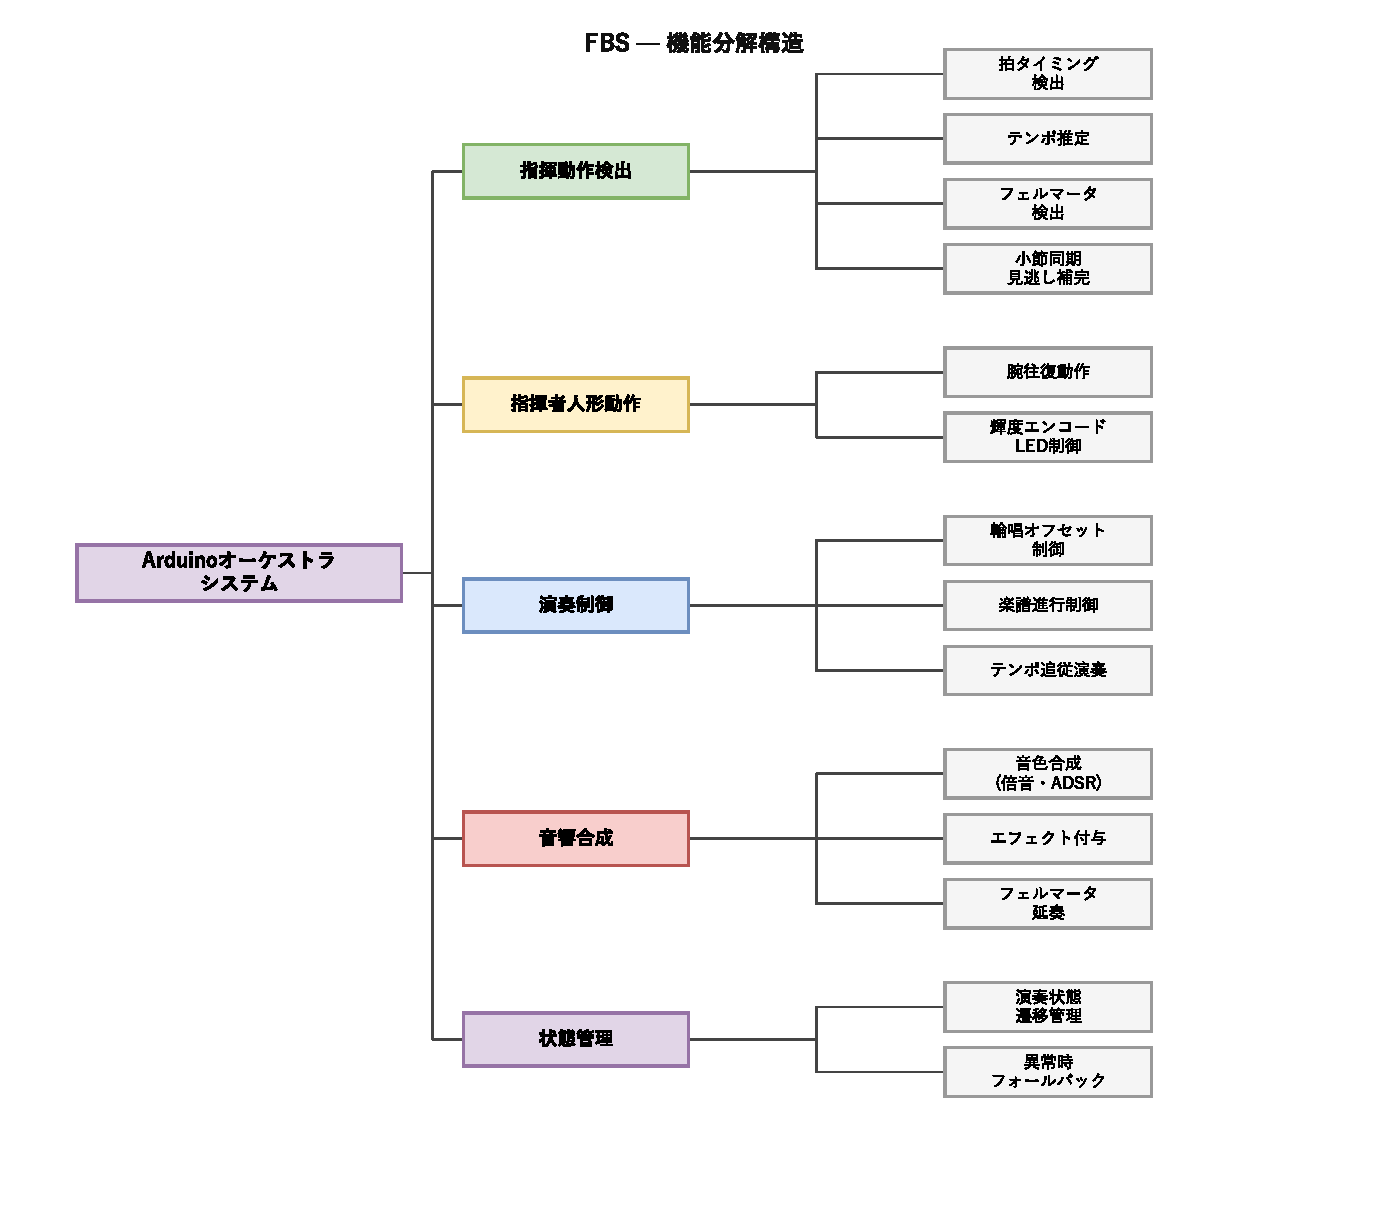
\includegraphics[width=\linewidth]{figures/common/fbs.drawio.pdf}
  \caption{機能分解構造（FBS）}
  \label{fig:fbs}
\end{figure}

\subsection{製品分解構造PBS}

製品分解構造（PBS：Product Breakdown Structure）は，システムを構成する成果物（ハードウェア・ソフトウェア・データ）を階層的に分解したものである．
本プロジェクトのPBSを図\ref{fig:pbs}に示す．

最上位（L0）を担当単位（L1）で分割し，各担当の成果物（L2）およびその構成要素（L3）まで展開する．

\begin{itemize}
  \item \textbf{担当A（指揮者人形ユニット）}：サーボ機構・腕・反射板からなる人形機構，カラーLED・サーボ駆動回路，およびサーボ制御・カラーLED制御ソフトウェア，ならびに楽器指定・BPM入力・演奏制御ボタンを備えたProcessing専用GUIインターフェース．
  \item \textbf{担当B（センサー・観測）}：フォトトランジスタ配線（遮光チャンバー含む），カラーセンサ配線，センサーISR・EMAテンポ推定・状態機械・カラーキュー判別を実装した観測Arduino SW．
  \item \textbf{担当C（演奏制御）}：カラーキュー受信・楽譜進行・シリアル送信を実装した演奏Arduino SW，および「かえるのうた」5パート分の楽譜配列データ．
  \item \textbf{担当D（音響合成）}：シリアル受信・音色合成エンジン・エフェクト処理を実装したProcessing SW，および音色定義シートとADSRパラメータからなる音色定義データ．
\end{itemize}

\begin{figure}[H]
  \centering
  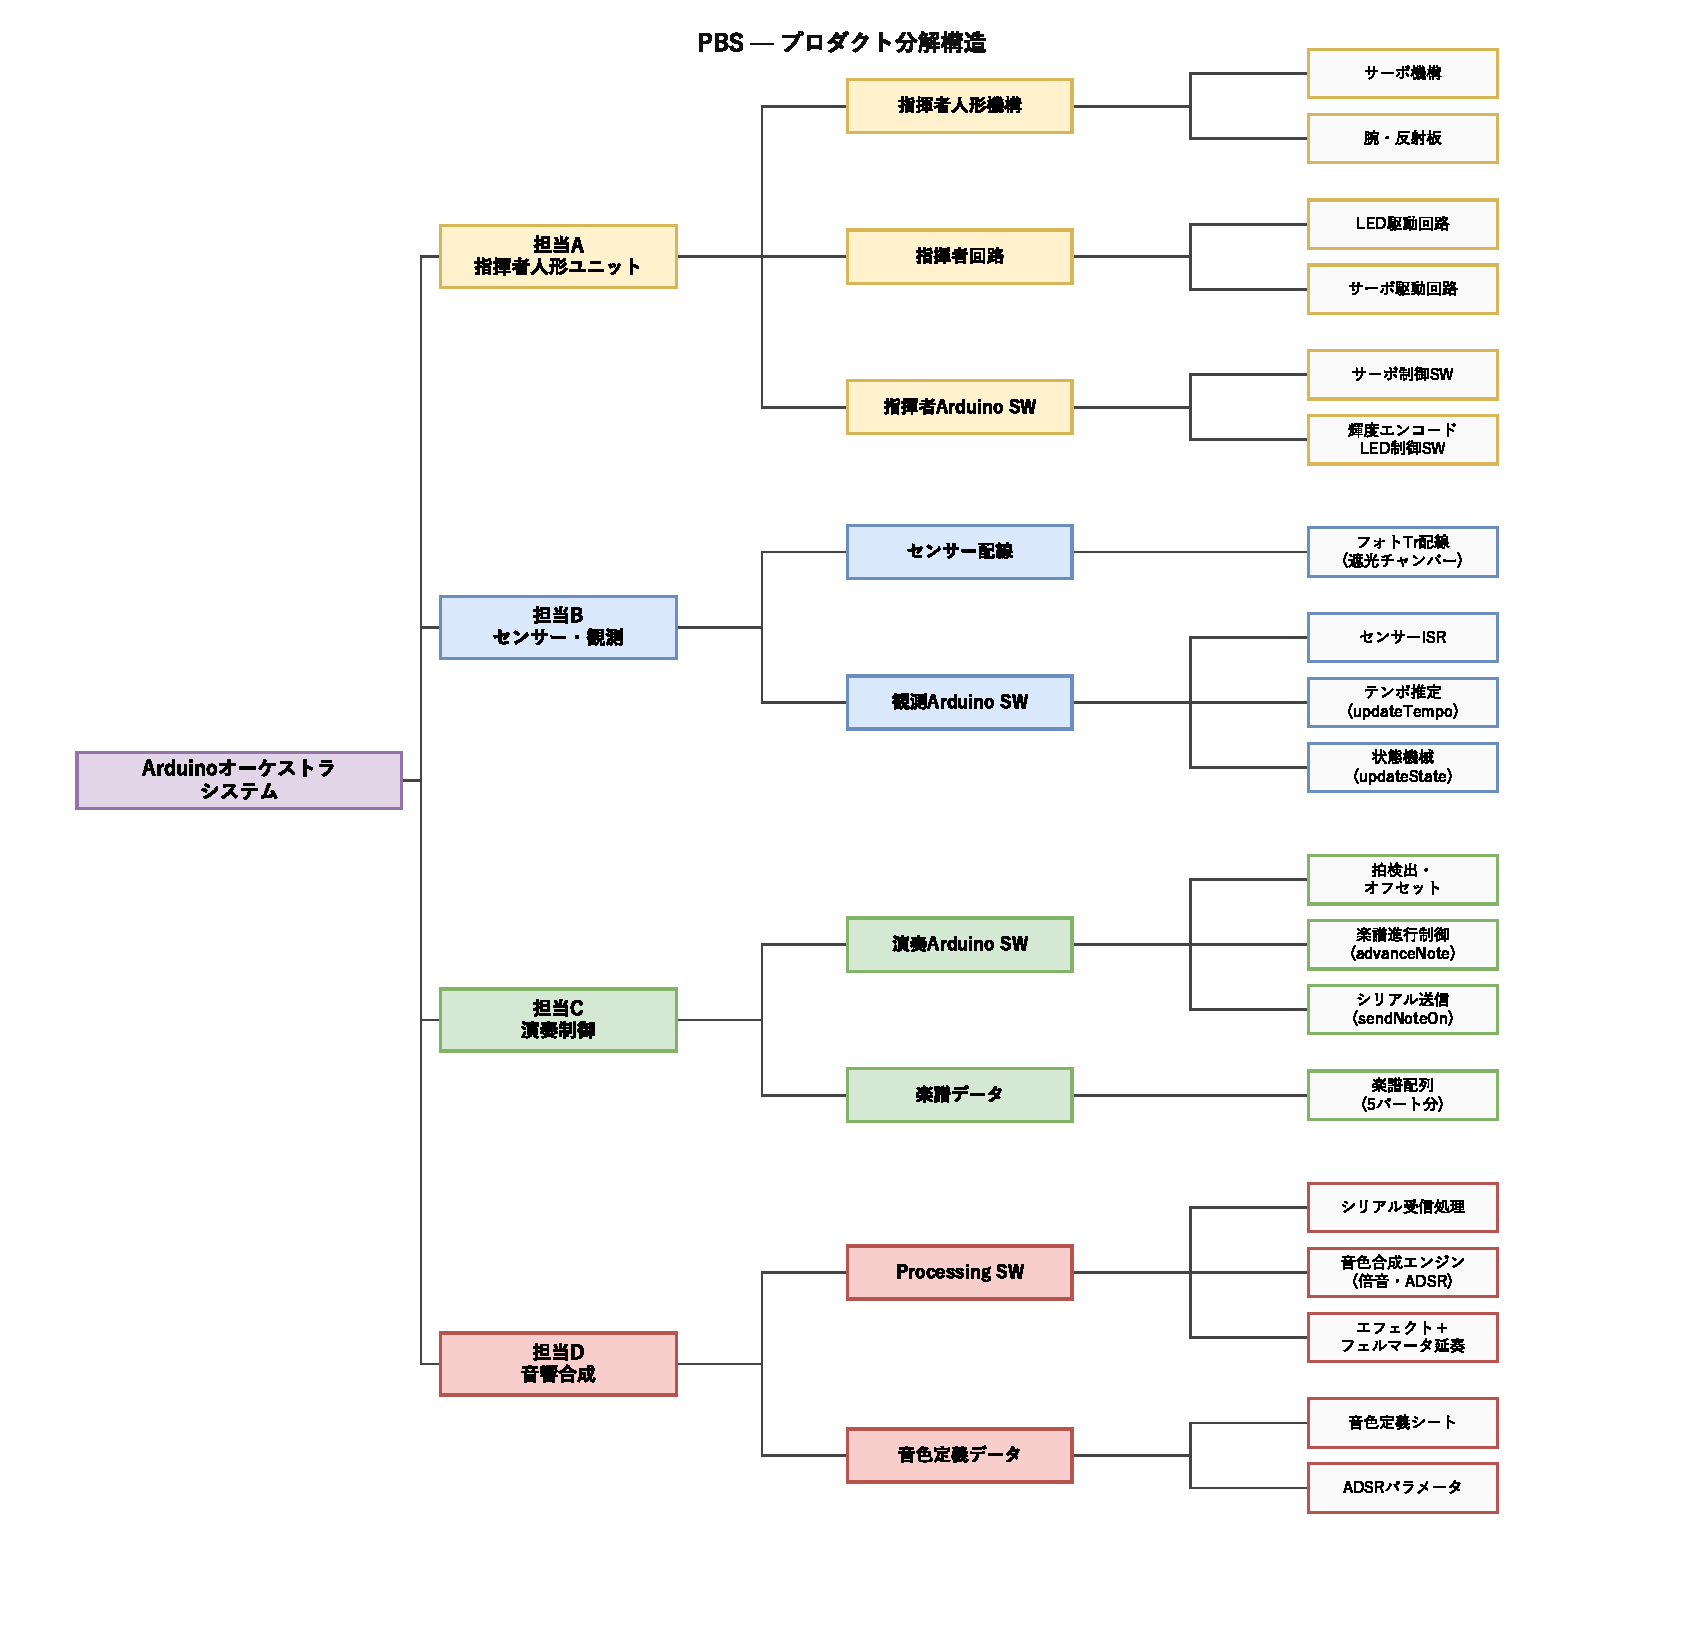
\includegraphics[width=\linewidth]{figures/common/pbs.drawio.pdf}
  \caption{製品分解構造（PBS）}
  \label{fig:pbs}
\end{figure}

\subsection{FBSとPBSの対応関係}

FBSの各機能とPBSの各成果物の対応関係を表\ref{tab:fbs-pbs}に示す．
FBSは「何をするか」，PBSは「何を作るか」を表しており，それぞれの機能は一つ以上の成果物によって実現される．

\begin{table}[H]
  \centering
  \caption{FBS機能とPBS成果物の対応}
  \label{tab:fbs-pbs}
  \begin{tabularx}{\linewidth}{lX}
    \toprule
    FBS機能（L2） & 対応するPBS成果物（L2/L3） \\
    \midrule
    拍タイミング検出    & センサー配線（フォトTr配線），観測Arduino SW（センサーISR） \\
    テンポ推定          & 観測Arduino SW（updateTempo） \\
    フェルマータ検出    & 観測Arduino SW（状態機械） \\
    小節同期・見逃し補完 & 観測Arduino SW（状態機械） \\
    \midrule
    腕往復動作          & 指揮者人形機構（サーボ機構・腕），指揮者回路（サーボ駆動回路），指揮者Arduino SW（サーボ制御SW） \\
    カラーLED制御 & 指揮者回路（カラーLED駆動回路），指揮者Arduino SW（カラーLED制御SW） \\
    \midrule
    演奏開始キュー制御  & カラーセンサ配線，観測Arduino SW（カラーキュー判別・開始フラグ管理） \\
    楽譜進行制御        & 演奏Arduino SW（advanceNote），楽譜データ（楽譜配列） \\
    テンポ追従演奏      & 演奏Arduino SW（sendNoteOn） \\
    \midrule
    音色合成            & Processing SW（音色合成エンジン），音色定義データ（音色定義シート・ADSRパラメータ） \\
    エフェクト付与      & Processing SW（エフェクト＋フェルマータ延奏） \\
    フェルマータ延奏    & Processing SW（エフェクト＋フェルマータ延奏） \\
    \midrule
    演奏状態遷移管理    & 観測Arduino SW（状態機械），Processing SW（シリアル受信処理） \\
    異常時フォールバック & 観測Arduino SW（状態機械） \\
    \bottomrule
  \end{tabularx}
\end{table}

% =====================
\section{作業計画}

\subsection{作業分解構造WBSと管理番号}
フェーズ100（設計），200（実装），300（テスト）の3フェーズで構成されるWBSを図\ref{fig:wbs}に示す．
各フェーズには複数の要素成果物と活動タスクが含まれ，それぞれに管理番号と担当者が割り当てられている．

\begin{figure}[H]
  \centering
  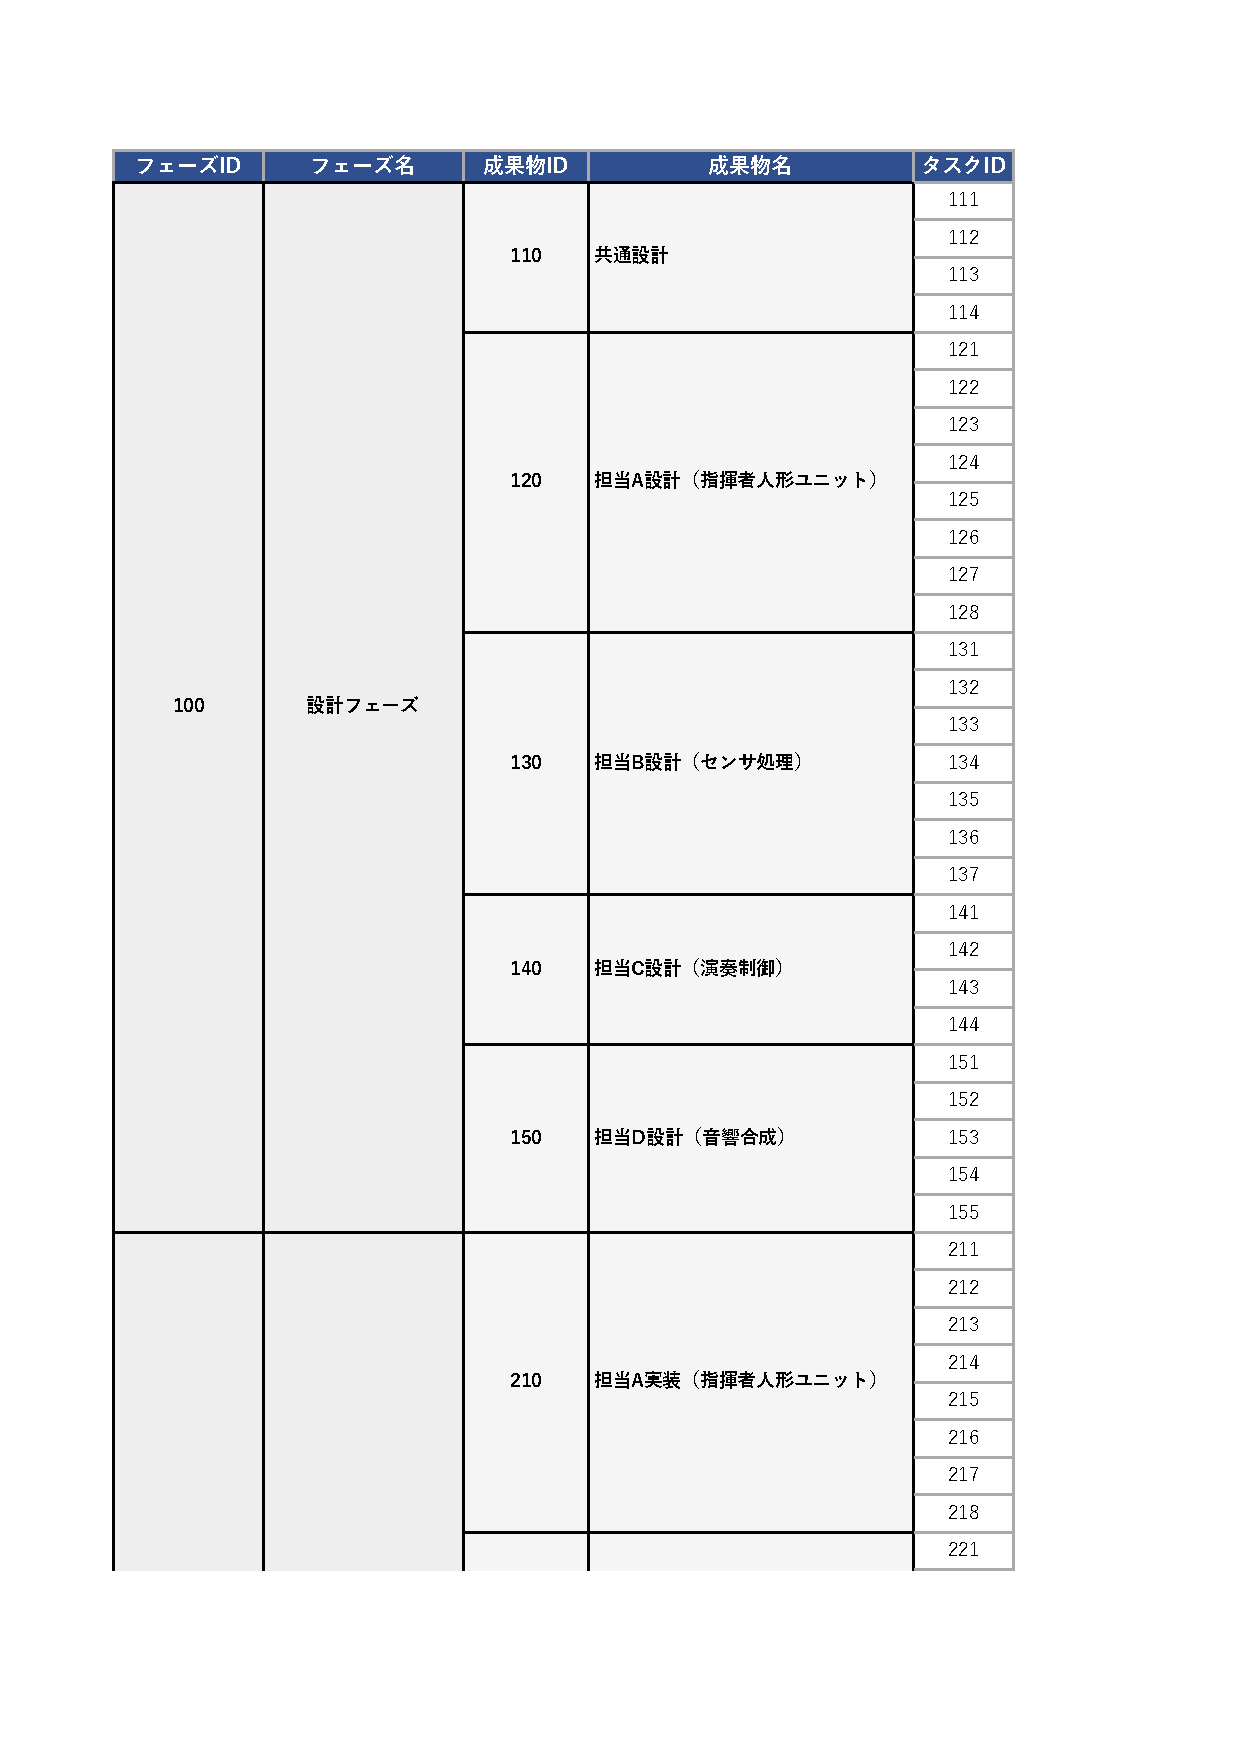
\includegraphics[width=\linewidth]{figures/common/wbs_v2.pdf}
  \caption{作業分解構造（WBS）}
  \label{fig:wbs}
\end{figure}

\subsection{アローダイアグラムとクリティカルパス}
アローダイアグラム（Activity on Arrow形式）を図\ref{fig:arrow}に示す．
各ノードには最早開始日（ES）と最遅開始日（LS）を記載し，
ES = LS となる活動をクリティカルパス（赤矢印）として示す．

\begin{figure}[H]
  \centering
  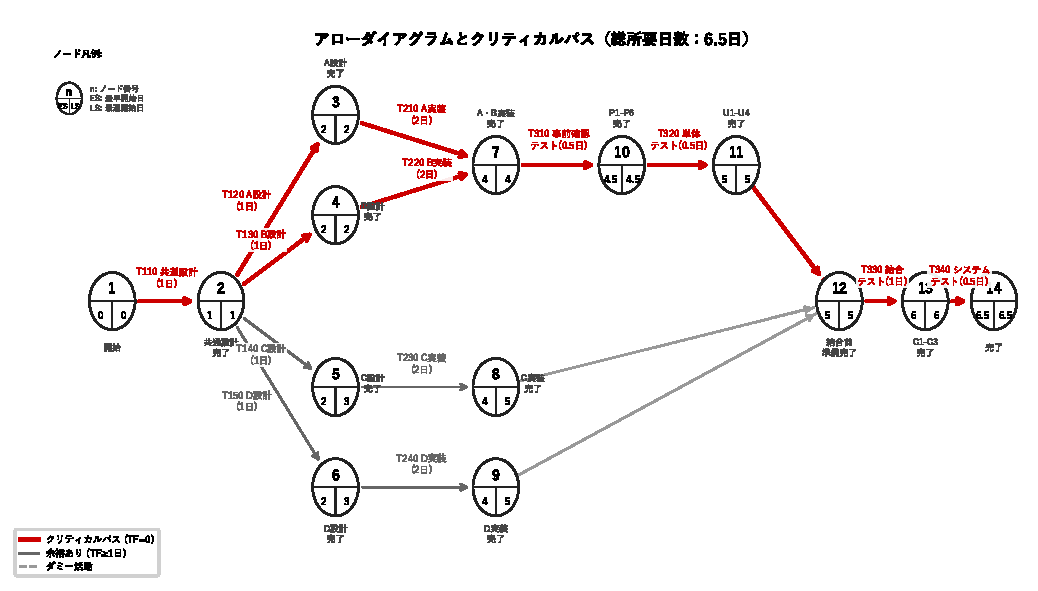
\includegraphics[width=\linewidth]{figures/common/arrow_diagram.pdf}
  \caption{アローダイアグラムとクリティカルパス}
  \label{fig:arrow}
\end{figure}

クリティカルパスは
$①\to②\to③\to⑦\to⑩\to⑪\to⑫\to⑬\to⑭$（担当A実装経由）
および
$①\to②\to④\to⑦\to⑩\to⑪\to⑫\to⑬\to⑭$（担当B実装経由）
の2経路であり，総所要日数は\textbf{6.5日}となる．
担当C・D（T140・T150・T230・T240）は各1日のトータルフロートを有する．

\subsection{役割分担}
WBS（図\ref{fig:wbs}）およびPBSに基づき，各機能およびコンポーネントの設計・実装・テストは以下の担当者に割り当てられている．

\begin{itemize}
  \item \textbf{担当A（指揮者人形ユニット）}：長見・飛田
  \item \textbf{担当B（センサー・観測）}：長野・慶田
  \item \textbf{担当C（演奏制御）}：長山・慶田
  \item \textbf{担当D（音響合成）}：中村・尾添
\end{itemize}

全体に関わる共通設計（WBS 110）や事前確認テスト以降の結合・システムテスト（WBS 300番台の一部）は，全員または関係する担当者が共同で実施する．

\subsection{ガントチャート}
図\ref{fig:gantt}にガントチャートを示す．
フェーズ200（実装）は第6週（5月18日）から各担当が並行して着手する．
第7週（5月25日）は大学のテスト期間に伴うバッファー週（薄橙色）として確保し，
実装作業を一時中断する．
フェーズ300（テスト）は第9週（6月8日）の事前確認テスト（P1--P6）から開始し，
単体テスト（U1--U4），結合テスト（C1--C3）を経て，
第11週（6月22日）のシステムテスト（S1--S3）で完了する．

\begin{figure}[H]
  \centering
  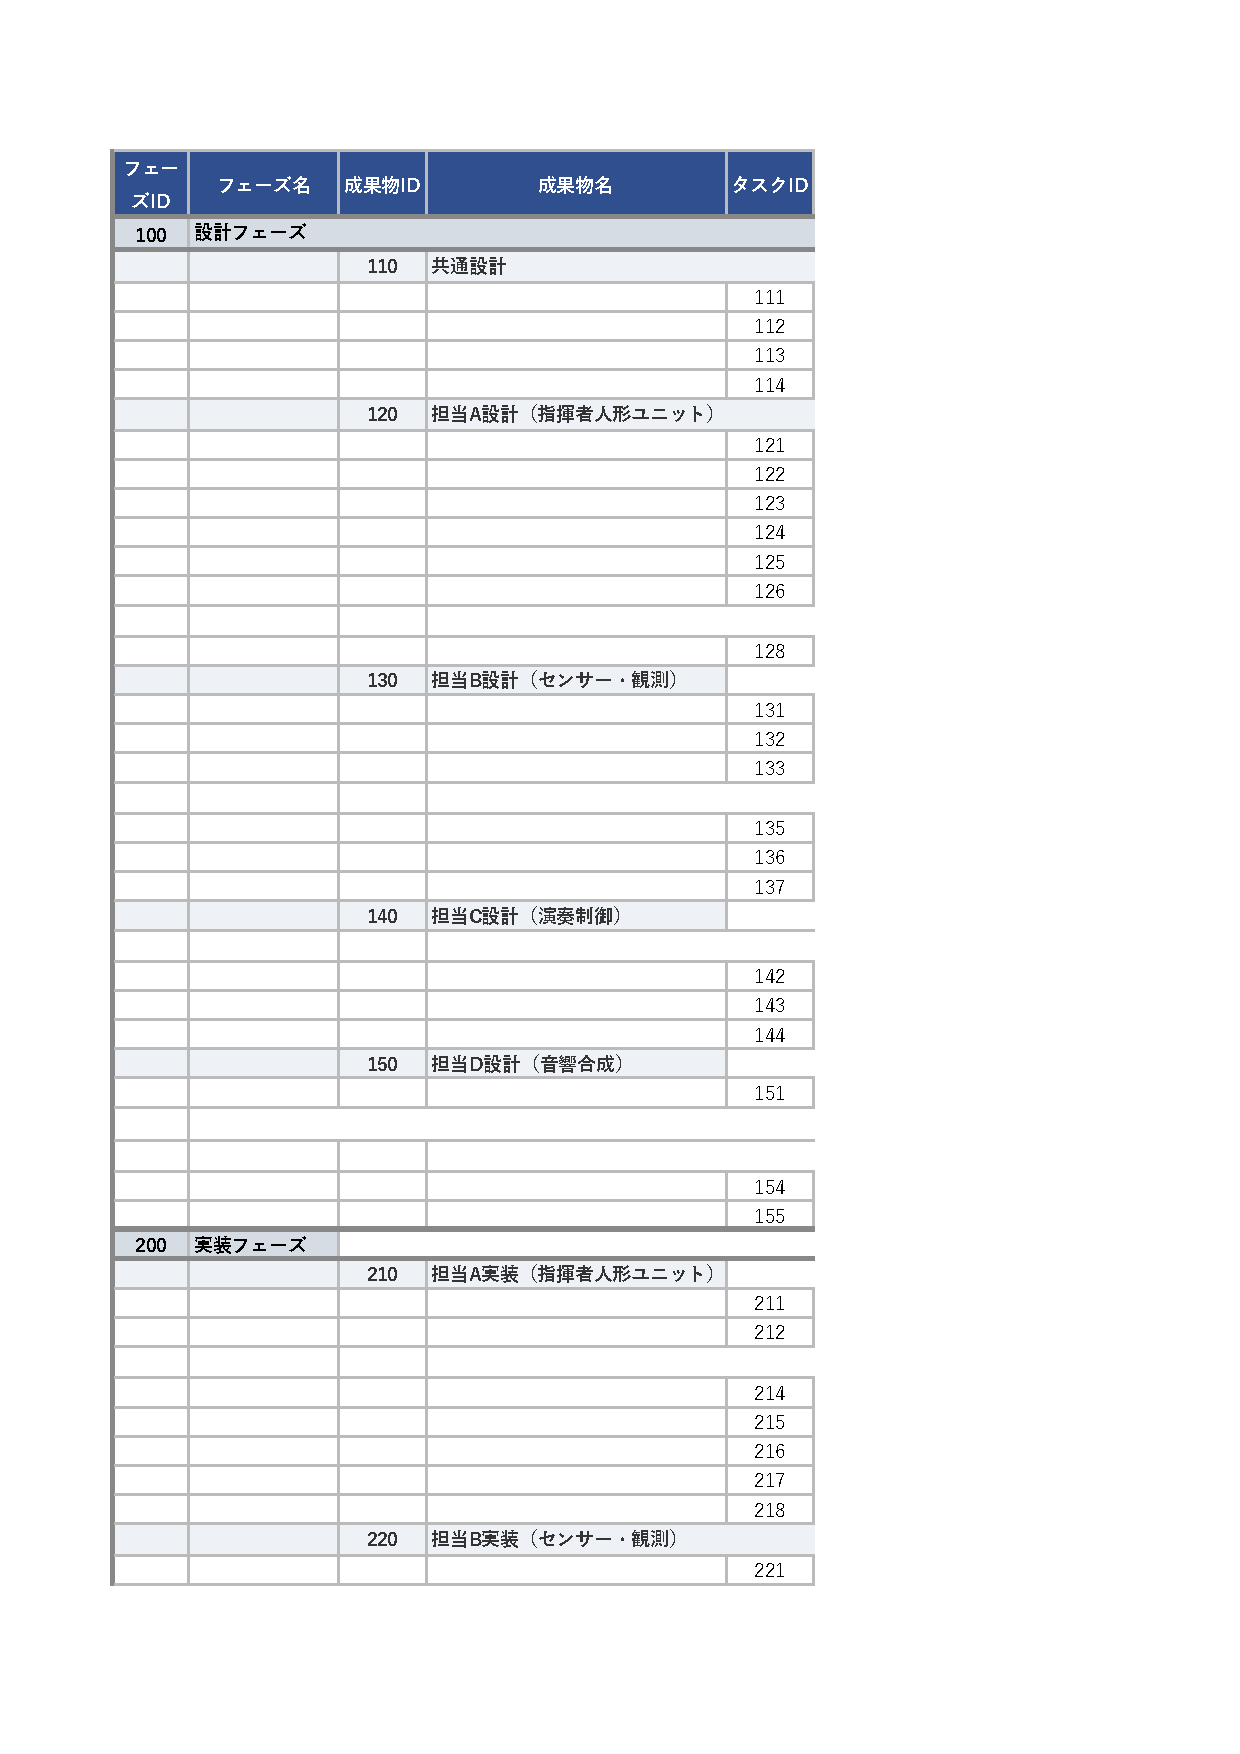
\includegraphics[width=\linewidth]{figures/common/gantt.pdf}
  \caption{ガントチャート}
  \label{fig:gantt}
\end{figure}

% =====================
\section{検証と妥当性確認：V\&V計画}

ハッカソン2テキスト§1.2.5に基づき，MOE → MOP → TPM の順で評価指標を定める．
実運用では順序が逆転し，実装中に TPM を継続監視し，
V\&V によって MOP を確認し，最終的に MOE で受入判定を行う．
本節では各指標の定義・数値目標・設定根拠を示す．
各MOPはスコープ・マネジメント節（§\ref{sec:scope}）で定めたFBSの機能要素に対応して設定している．
各MOPの具体的なテスト手順・判定基準は，第3章（システムの詳細設計）の
各担当節に設けたテスト設計（§3.1〜§3.4）に記述する．

\subsection{プロジェクトの成果物に対する有効指標MOE}

MOE（Measure of Effectiveness：有効指標）は，
ステークホルダ（審査員・聴衆）が成果物の合格・不合格を判定するための指標であり，
受入テストの合否基準に相当する．
本プロジェクトのMOEを表\ref{tab:moe}に示す．

\begin{table}[H]
  \centering
  \caption{MOE一覧}
  \label{tab:moe}
  \begin{tabularx}{\linewidth}{clXl}
    \toprule
    No. & MOE & 内容 & 確認方法 \\
    \midrule
    MOE-1 & 演奏完走 &
      「かえるのうた」5パート輪唱（テンポ変化・フェルマータ含む）を
      最初から最後まで演奏できること &
      実演で確認 \\
    MOE-2 & 指揮追従 &
      指揮者人形のテンポ変化・フェルマータに対して
      演奏が連動していることが視聴覚的に確認できること &
      審査員観察評価 \\
    MOE-3 & 楽器音認識 &
      各パートが意図した楽器（ピアノ・鉄琴・トランペット・
      バス/スネア・ハイハット）の音として聴こえること &
      審査員主観評価 \\
    \bottomrule
  \end{tabularx}
\end{table}

表\ref{tab:moe}に示すように，MOEはMOE-1（演奏完走）・MOE-2（指揮追従）・MOE-3（楽器音認識）の3項目からなる．
MOE-1は本システムの最低限の動作要件であり，演奏が途中で止まることは致命的な失敗にあたるため設定した．
MOE-2は本システムの独自性である「指揮者人形の観測による自律同期」が実際に機能しているかを
聴衆・審査員が知覚できることを確認するために設定した．
MOE-3はProcessingによる音響合成の品質を評価するために設定した．

\subsection{有効指標MOEに対応する性能指標MOP}

MOP（Measure of Performance：性能指標）はMOEを達成するために必要な
システム性能を定量的に示す指標であり，V字モデルの設計段階で定義する．
FBSの各機能に対応する性能要素に対して設定したMOPと，
対応するMOEを表\ref{tab:moe-mop}に示す．

\begin{table}[H]
  \centering
  \caption{MOEとMOPの対応}
  \label{tab:moe-mop}
  \begin{tabularx}{\linewidth}{clX}
    \toprule
    No. & 対応MOE & MOP \\
    \midrule
    1 & MOE-1,2 & フォトトランジスタによる拍検出成功率 \\
    2 & MOE-1,2 & 楽器間の発音タイミング誤差 \\
    3 & MOE-1,2 & テンポ変化後のEMA収束拍数 \\
    4 & MOE-1,2 & 腕停止からフェルマータ状態移行までの拍数 \\
    5 & MOE-3   & 各パートの発音周波数精度 \\
    \bottomrule
  \end{tabularx}
\end{table}

表\ref{tab:moe-mop}に示すMOPはそれぞれMOE-1・MOE-2の達成に関わる技術的な性能要素であり，
各テストフェーズにおいて数値目標として評価する．
具体的な目標値はシステムテスト・結合テスト・単体テストの各節で示す．

\subsection{システムテストで評価する性能指標MOP}

システム全体を統合した状態で評価するMOPを表\ref{tab:mop-sys}に示す．

\begin{table}[H]
  \centering
  \caption{システムテストで評価するMOP}
  \label{tab:mop-sys}
  \begin{tabularx}{\linewidth}{llX}
    \toprule
    No. & 対応FBS機能 & MOP（目標値） \\
    \midrule
    SYS-1 & テンポ推定 &
      テンポ変化後の収束：$\leq 3$拍 \\
    SYS-2 & フェルマータ検出 &
      腕停止からフェルマータ移行：$\leq 1$拍 \\
    SYS-3 & 楽譜進行制御 &
      全区間通し演奏の完走率：$100\,\%$ \\
    \bottomrule
  \end{tabularx}
\end{table}

表\ref{tab:mop-sys}に示す各MOPの目標値の設定根拠を以下に示す．

SYS-1の目標値3拍の根拠を示す．
本楽曲「かえるのうた」は4/4拍子（1小節=4拍）で演奏される．
EMAの更新式は$T_n = \alpha \cdot \Delta t_n + (1-\alpha)\cdot T_{n-1}$であり，
テンポ変化後の残差は$(1-\alpha)^n$で減衰する．
テンポ変化を検出した際の平滑化係数$\alpha=0.5$を用いると，
$n$拍後の残差は$0.5^n$となり，$n=3$のとき$0.5^3=0.125$（87.5\%収束）である．
4/4拍子において，テンポ変化後に1小節未満（$\leq 3$拍）で収束すれば，
次の小節の先頭から新テンポで各楽器が揃って演奏を再開できる．
この「次小節頭で揃う」という音楽的要件と$\alpha=0.5$のEMA特性の両面から，
$\leq 3$拍を目標値とした．

SYS-2の目標値1拍の根拠を示す．
フェルマータは楽譜上で特定の拍に付与される記号であり，
腕停止を検出してから1拍以上経過すると，その拍の音符が余分に発音されて旋律が崩れる．
したがって，腕停止検出から次の拍が来る前にフェルマータ状態へ移行しなければならず，
この楽譜上の制約から$\leq 1$拍を上限として設定した．
フェルマータ検出の具体的な実装はFBS機能F2a4（フェルマータ検出）に対応し，
詳細は担当Bの詳細設計（第3章§3.2）に記述する．

SYS-3の100\%はMOE-1（演奏完走）の定義そのものであり，
システムテストの合格条件として妥協のない値として設定した．

なお，各システムテストの実施手順・判定基準は第3章の各担当詳細設計節に記述する．

\subsection{結合テストで評価する性能指標MOP}

複数の担当成果物を結合した状態で評価するMOPを表\ref{tab:mop-int}に示す．

\begin{table}[H]
  \centering
  \caption{結合テストで評価するMOP}
  \label{tab:mop-int}
  \begin{tabularx}{\linewidth}{llX}
    \toprule
    No. & 対応FBS機能 & MOP（目標値） \\
    \midrule
    INT-1 & テンポ追従演奏 &
      楽器間発音タイミング誤差：$\leq \pm 20\,\mathrm{ms}$ \\
    INT-2 & テンポ追従演奏 &
      Arduino→Processing転送遅延：$\leq 50\,\mathrm{ms}$ \\
    INT-3 & 輪唱オフセット制御 &
      輪唱オフセット誤差：$\leq \pm 1$拍 \\
    \bottomrule
  \end{tabularx}
\end{table}

表\ref{tab:mop-int}に示す各MOPの設定根拠を以下に示す．
INT-1の目標値$\pm 20\,\mathrm{ms}$は，人間が音楽的なタイミングのズレを知覚できる
閾値（先行研究では概ね$20\sim30\,\mathrm{ms}$\cite{sudo2007,kawase}）の下限値を採用した．
INT-2の目標値$50\,\mathrm{ms}$の根拠を示す．
115200\,bpsのシリアル通信では，スタート・データ8bit・ストップビットを含む1バイト=10bitを送信する．
3バイトパケットの純粋な転送時間は$\frac{3 \times 10}{115200} \approx 0.26\,\mathrm{ms}$である．
これにProcessing側のバッファ読み取り間隔（典型10\,ms未満）を加えても実測値は数ms程度であり，
$50\,\mathrm{ms}$は十分な余裕を持った上限値である．
また，各楽器ユニットで遅延が一定であれば遅延補正値で吸収できるため，絶対値よりも安定性が重要である．

INT-3の目標値$\pm 1$拍の根拠を示す．
輪唱は各パートが一定拍数ずれて同じ旋律を演奏する構造であり，
オフセットが$\pm 1$拍以上ずれると隣接パートの音符と重なり旋律が崩れる．
したがって輪唱として成立する最小単位である「1拍」をそのまま上限として設定した．

なお，結合テストの具体的な実施手順・タイムスタンプ計測方法は，
担当B・Cの詳細設計（第3章§3.2・§3.3）に記述する．

\subsection{単体テストで評価する性能指標MOP}

各担当成果物を単独で評価する単体テストのMOPを表\ref{tab:mop-unit}に示す．

\begin{table}[H]
  \centering
  \caption{単体テストで評価するMOP}
  \label{tab:mop-unit}
  \begin{tabularx}{\linewidth}{lX}
    \toprule
    No. & MOP（目標値） \\
    \midrule
    UNIT-1 & 拍検出成功率：$\geq 95\,\%$ \\
    UNIT-2 & 距離計算誤差：$\leq \pm 3\,\mathrm{cm}$ \\
    UNIT-3 & EMA通常演奏時（$\alpha=0.2$）の収束：$\leq 13$拍 \\
    UNIT-4 & NOTE\_ON送信タイミング誤差：$\leq \pm 10\,\mathrm{ms}$ \\
    UNIT-5 & 発音周波数精度：目標周波数の$\pm 1\,\mathrm{Hz}$以内 \\
    UNIT-6 & BPM追従誤差：$\leq \pm 5\,\mathrm{bpm}$ \\
    UNIT-7 & ストローク変動：$\leq \pm 2\,\mathrm{mm}$ \\
    \bottomrule
  \end{tabularx}
\end{table}

表\ref{tab:mop-unit}に示す各MOPの設定根拠を以下に示す．

UNIT-1の目標値95\%の根拠を示す．
検出失敗率を$p = 1 - 0.95 = 0.05$とすると，3拍連続で失敗する確率は
$p^3 = 0.05^3 = 1.25 \times 10^{-4}$（約0.013\%）である．
フォールバック処理は3拍連続未検出で発動するため，
検出成功率95\%を維持すればフォールバックがほぼ発動しないことが保証される．

UNIT-2の目標値$\pm 3\,\mathrm{cm}$の根拠を示す．
フェルマータ検出は絶対距離ではなく腕の「変化量」$\Delta d$で判定するため，
絶対距離の精度要件は緩やかである．
センサー出力電圧$V$から距離$d$を推定する近似式$d = 27.728 \times V^{-1.2045}$において，
ArduinoのAD変換（10bit，5\,V系）の量子化誤差$\Delta V \approx 5/1024 \approx 4.9\,\mathrm{mV}$を伝搬させると，
$d \approx 30\,\mathrm{cm}$付近での距離誤差は数mm〜数cm程度となる．
この誤差範囲を包含する上限として$\pm 3\,\mathrm{cm}$を設定した．

UNIT-3の目標値13拍の根拠を示す．
$\alpha=0.2$のEMAが95\%収束（残差$\leq 5\%$）するのに必要な拍数は，
$(1-\alpha)^n \leq 0.05$を解いて
$n \geq \frac{\ln 0.05}{\ln(1-\alpha)} = \frac{\ln 0.05}{\ln 0.8} \approx 13.4$拍，
切り上げで14拍となる．
14拍以内に収束することを確認するため，余裕を1拍見て13拍を確認目標とした．

UNIT-4の目標値$\pm 10\,\mathrm{ms}$の根拠を示す．
楽器間タイミング誤差（INT-1：$\pm 20\,\mathrm{ms}$）は，
各楽器の送信誤差が独立に重なった合計で生じる．
最悪ケースで2つの楽器が逆方向に最大誤差を持つと，
$(\pm 10) - (\pm 10) = \pm 20\,\mathrm{ms}$となる．
よって，各楽器単体の誤差をINT-1の半分である$\pm 10\,\mathrm{ms}$以内に抑えることでINT-1を満たせる．

UNIT-5の目標値$\pm 1\,\mathrm{Hz}$は，音楽的に許容されるピッチのずれ（約$\pm 5\,\mathrm{cent}$，
A4=440\,Hzで約$\pm 1.3\,\mathrm{Hz}$\cite{jnd1974}）に対して余裕を持たせた値である．

UNIT-6の目標値$\leq \pm 5\,\mathrm{bpm}$の根拠を示す．
80\,bpmを基準テンポとすると，1拍の周期は$60/80 = 750\,\mathrm{ms}$である．
人間がテンポ変化を知覚できる閾値は一般に約3〜6\%とされており，
80\,bpmの6\%は$80 \times 0.06 = 4.8\,\mathrm{bpm}$である．
この値を切り上げた$\pm 5\,\mathrm{bpm}$を，聴衆が追従と判断できる上限として設定した．

UNIT-7の目標値$\leq \pm 2\,\mathrm{mm}$の根拠を示す．
指揮者人形のストローク幅はEMA（担当B）が計算する「振り幅」に対応し，
ストローク変動が大きいとBPM推定の誤差（UNIT-6）に直接影響する．
UNIT-6の目標値$\leq \pm 5\,\mathrm{bpm}$を80\,bpmにおける1拍周期の変動量に換算すると，
$\Delta T = 60/80 - 60/85 \approx 44\,\mathrm{ms}$であり，
これを引き起こすストローク誤差は機構設計（担当A詳細設計§3.1）の寸法から$\pm 2\,\mathrm{mm}$以内と見積もられる．

各単体テストの具体的な実施手順は，第3章の各担当詳細設計節
（担当A：§3.1，担当B：§3.2，担当C：§3.3，担当D：§3.4）のテスト設計に記述する．

\subsection{プロジェクト中に監視する技術性能指標TPM}

TPM（Technical Performance Measure：技術性能指標）は，開発・実装中に
継続的に測定・報告する定量的指標であり，技術的リスクの早期発見を目的とする．
MOPのうち特にシステム完成時の性能に大きく影響し，
実装の早い段階から測定できる項目を選定した．
TPM一覧を表\ref{tab:tpm}に示す．

\begin{table}[H]
  \centering
  \caption{TPM一覧}
  \label{tab:tpm}
  \begin{tabularx}{\linewidth}{lX}
    \toprule
    No. & TPM（監視値・許容範囲） \\
    \midrule
    TPM-1 & 距離計算誤差：$\leq \pm 3\,\mathrm{cm}$ \\
    TPM-2 & 拍検出成功率：$\geq 95\,\%$ \\
    TPM-3 & Arduino→Processing転送遅延：$\leq 50\,\mathrm{ms}$ \\
    TPM-4 & EMA（$\alpha=0.2$）テンポ収束拍数：$\leq 13$拍 \\
    TPM-5 & 指揮者人形が追従できる最大BPM：$\geq 104\,\mathrm{bpm}$ \\
    TPM-6 & テンポ予測誤差（予測拍時刻と実測拍時刻の差）：$\leq 1\,\mathrm{ms}$ \\
    \bottomrule
  \end{tabularx}
\end{table}

\subsection{TPMの監視体制}

表\ref{tab:tpm-monitor}に，各TPMの監視方法を示す．
監視方法の詳細（使用機材・記録フォーマット）は第3章各担当詳細設計節のテスト設計に記述する．

\begin{table}[H]
  \centering
  \caption{TPM監視体制}
  \label{tab:tpm-monitor}
  \begin{tabularx}{\linewidth}{lX}
    \toprule
    TPM & 監視方法 \\
    \midrule
    TPM-1 & 既知距離での実測値と近似式の計算値を比較し誤差を記録する \\
    TPM-2 & メトロノームに合わせた指揮動作でフォトTrの検出率をシリアルモニタで計測する \\
    TPM-3 & Arduino側の送信タイムスタンプとProcessing側の受信タイムスタンプの差分を計測・記録する \\
    TPM-4 & 既知BPMのシミュレーションデータを入力してEMAの収束拍数を計測する \\
    TPM-5 & 指定BPMで指揮者人形を動作させ，脱調・遅延の有無をシリアルモニタで確認する \\
    TPM-6 & シリアルモニタで予測拍時刻と実測拍時刻の差を100回計測し，平均誤差を記録する \\
    \bottomrule
  \end{tabularx}
\end{table}

% =====================
\section{資源・調達管理}

\subsection{人的資源}

本プロジェクトの人的資源は7名のメンバーで構成される．
各メンバーは担当A〜Dのいずれかに所属し，設計・実装・テストの全工程を通じてその担当領域を主体的に推進する（表\ref{tab:human-resource}）．

\begin{table}[H]
  \centering
  \caption{人的資源一覧}
  \label{tab:human-resource}
  \begin{tabularx}{\linewidth}{llX}
    \toprule
    担当 & メンバー & 主な責務 \\
    \midrule
    A（指揮者人形ユニット） & 長見・飛田 & 人形機構組み立て，LED・サーボ駆動回路，サーボ制御SW \\
    B（センサー・観測）     & 長野・慶田 & センサー配線，センサーISR・EMAテンポ推定・状態機械SW \\
    C（演奏制御）           & 長山・慶田 & 楽譜配列作成，拍検出・楽譜進行・シリアル送信SW \\
    D（音響合成）           & 中村・尾添 & 音色定義データ，音色合成エンジン・エフェクトProcessing SW \\
    \bottomrule
  \end{tabularx}
\end{table}

共通設計（WBS 110）および結合・システムテスト（WBS 330・340）は全員または関係担当者が共同で実施し，特定担当に過負荷が集中しないよう調整する．

\subsection{機材・調達計画}

本プロジェクトで必要なハードウェア機材を表\ref{tab:procurement}に示す．
実験室に常備されている機材（既備）は追加調達不要とし，不足分のみを授業実施機関に申請または自費で調達する．

\begin{table}[H]
  \centering
  \caption{機材・調達計画}
  \label{tab:procurement}
  \begin{tabularx}{\linewidth}{Xlcc}
    \toprule
    機材名 & 用途 & 数量 & 調達区分 \\
    \midrule
    Arduino Uno R4 WiFi & 指揮者・観測・演奏各制御 & 6 & 既備 \\
    サーボモータ（SG92R） & 指揮者人形の腕往復動作 & 1 & 既備 \\
    赤外線距離センサ（Sharp GP2Y0A21YK） & 腕位置連続観測 & 5 & 既備 \\
    フォトトランジスタ & 指揮者LED発光の拍検出 & 5 & 既備 \\
    高輝度LED（赤外線） & 指揮者側拍通知光源 & 2 & 既備 \\
    抵抗・コンデンサ類 & 各回路の定数設定 & 適量 & 既備 \\
    ブレッドボード・ジャンパ線 & プロトタイプ配線 & 適量 & 既備 \\
    スピーカ（パッシブ）& Processing音声出力 & 5 & 既備 \\
    工作材料（段ボール・スポンジ等） & 人形機構・遮光チャンバー筐体 & 適量 & 申請調達 \\
    PC（Processing実行用） & 音響合成・シリアル受信 & 6 & 持ち込み \\
    \bottomrule
  \end{tabularx}
\end{table}

調達が必要な物品（工作材料）は第5週（5月11日）までに申請を完了し，
第6週（5月18日）の実装開始に間に合うよう手配する．
電子部品は実験室常備品で賄えない場合のみ，担当Aが第5週中に代替品の確認および申請を行う．

\subsection{開発環境}

本プロジェクトで使用するソフトウェア開発環境を以下に示す．
いずれも無償利用可能なツールであり，追加ライセンス費用は発生しない．

\begin{itemize}
  \item \textbf{Arduino IDE 2.x}：ArduinoのSW開発・書き込み（担当A・B・C）
  \item \textbf{Processing 4.x}：音響合成SWの開発・実行（担当D）
  \item \textbf{draw.io}：FBS・PBS・WBS図の作成・管理（全員）
  \item \textbf{Git / GitHub}：ソースコードのバージョン管理（全員）
  \item \textbf{LuaLaTeX / jlreq}：本計画書・設計書のドキュメント作成（全員）
\end{itemize}

% =====================
\section{リスク管理}

\subsection{リスクの識別と評価}

プロジェクト遂行上のリスクを識別し，発生確率（H/M/L）と影響度（H/M/L）の組み合わせでリスクレベルを評価した結果を表\ref{tab:risk}に示す．

\begin{table}[H]
  \centering
  \caption{リスク一覧と評価}
  \label{tab:risk}
  \begin{tabularx}{\linewidth}{clXcc}
    \toprule
    No. & リスク名 & 内容 & 確率 & 影響 \\
    \midrule
    R-1 & センサー精度不足 &
      フォトTr・赤外線センサが要求精度（UNIT-1：95\%，UNIT-2：$\pm3\,$cm）を
      達成できず，拍検出やフェルマータ検出が不安定になる &
      M & H \\
    R-2 & サーボ最大BPM不足 &
      SG90のトルク・応答速度が不足し，目標最大BPM（TPM-5：104\,bpm）で
      脱調または動作遅延が生じる &
      M & M \\
    R-3 & EMAチューニング失敗 &
      $\alpha$の値が適切に調整できず，テンポ収束（SYS-1：$\leq3$拍）や
      フェルマータ検出（SYS-2：$\leq1$拍）が達成できない &
      M & H \\
    R-4 & 通信遅延超過 &
      Arduino→Processing間のシリアル遅延がINT-2（$\leq50\,$ms）を
      超え，発音タイミングがずれる &
      L & M \\
    R-5 & 機材調達遅延 &
      3Dプリント材料等の申請承認が遅れ，第6週の実装開始が遅延する &
      L & H \\
    R-6 & スケジュール圧迫 &
      各担当の実装が第8週までに完了せず，第9週からのテストフェーズが
      縮小または中止になる &
      M & H \\
    R-7 & 遮光チャンバー性能不足 &
      外乱光によりフォトTrが誤検出し，拍検出成功率（UNIT-1）が低下する &
      M & M \\
    \bottomrule
  \end{tabularx}
\end{table}

\subsection{リスク対応計画}

表\ref{tab:risk}で識別した各リスクに対する対応策を表\ref{tab:risk-response}に示す．

\begin{table}[H]
  \centering
  \caption{リスク対応計画}
  \label{tab:risk-response}
  \small
  \begin{tabularx}{\linewidth}{clXX}
    \toprule
    No. & リスク名 & 対応策（軽減/回避/受容） & トリガー条件 \\
    \midrule
    R-1 & センサー精度不足 &
      【軽減】事前確認テスト（P1--P3）でセンサー単体精度を第9週頭に検証し，
      不足時はセンサー取り付け位置・遮光調整または閾値再設定を行う &
      UNIT-1$<$95\%またはUNIT-2$>\pm3\,$cm \\
    R-2 & サーボ最大BPM不足 &
      【軽減】事前確認テスト（P4--P5）でサーボ最大BPMを実測し，
      不足時は腕のストローク角度を縮小して応答速度を確保する &
      TPM-5$<$104\,bpm \\
    R-3 & EMAチューニング失敗 &
      【軽減】シミュレーションデータによる単体テスト（U1）でEMAの
      収束特性を事前検証し，$\alpha$を段階的に調整して目標範囲内に収める &
      収束拍数$>$3拍またはフェルマータ移行$>$1拍 \\
    R-4 & 通信遅延超過 &
      【受容・軽減】115200\,bpsの遅延は理論上1\,ms未満であり発生確率は低い．
      万一超過した場合はバッファ読み取り処理をPollingからイベント駆動に変更する &
      TPM-3$>$50\,ms \\
    R-5 & 機材調達遅延 &
      【回避】第5週（5月11日）中に申請を完了し，承認が遅れる場合は
      手持ちの材料で代替した簡易筐体を先行して製作する &
      第6週開始時点で材料未着 \\
    R-6 & スケジュール圧迫 &
      【軽減】第7週のバッファー週を活用して遅延分を吸収する．
      それでも遅延が残る場合は，未完了タスクをテストフェーズ前半（第9週）に繰り越し，
      テストスコープを縮小して対応する &
      第8週末時点で実装完了率$<$90\% \\
    R-7 & 遮光チャンバー性能不足 &
      【軽減】遮光チャンバーに黒色テープ・フォームを追加して外乱光を遮断する．
      それでも改善しない場合はフォトTrをシールドケースに封入する &
      屋内通常照明下でUNIT-1$<$95\% \\
    \bottomrule
  \end{tabularx}
\end{table}

\subsection{リスク監視体制}

各担当は週次のミーティング（授業時間内）にTPMの計測結果を報告し，
表\ref{tab:risk}のトリガー条件に抵触したリスクが発生した場合は
その場で対応策の着手を決定する．
リスクレベルがH×H（高確率かつ高影響）に達した場合は全員でスコープの再確認を行い，
MOE-1（演奏完走）の達成を最優先として成果物を取捨選択する．
